%% This is file `elsarticle-template-1-num.tex',
%%
%% Copyright 2009 Elsevier Ltd
%%
%% This file is part of the 'Elsarticle Bundle'.
%% ---------------------------------------------
%%
%% It may be distributed under the conditions of the LaTeX Project Public
%% License, either version 1.2 of this license or (at your option) any
%% later version.  The latest version of this license is in
%%    http://www.latex-project.org/lppl.txt
%% and version 1.2 or later is part of all distributions of LaTeX
%% version 1999/12/01 or later.
%%
%% Template article for Elsevier's document class `elsarticle'
%% with numbered style bibliographic references
%%
%% $Id: elsarticle-template-1-num.tex 149 2009-10-08 05:01:15Z rishi $
%% $URL: http://lenova.river-valley.com/svn/elsbst/trunk/elsarticle-template-1-num.tex $
%%
\documentclass[preprint,12pt]{elsarticle}

%% Use the option review to obtain double line spacing
%% \documentclass[preprint,review,12pt]{elsarticle}

%% Use the options 1p,twocolumn; 3p; 3p,twocolumn; 5p; or 5p,twocolumn
%% for a journal layout:
%% \documentclass[final,1p,times]{elsarticle}
%% \documentclass[final,1p,times,twocolumn]{elsarticle}
%% \documentclass[final,3p,times]{elsarticle}
%% \documentclass[final,3p,times,twocolumn]{elsarticle}
%% \documentclass[final,5p,times]{elsarticle}
%% \documentclass[final,5p,times,twocolumn]{elsarticle}

%% The graphicx package provides the includegraphics command.
\usepackage{graphicx}
%% The amssymb package provides various useful mathematical symbols
\usepackage{amssymb} 
\usepackage{amsmath}
\usepackage{amssymb}
%% The amsthm package provides extended theorem environments
%% \usepackage{amsthm}

%% The lineno packages adds line numbers. Start line numbering with
%% \begin{linenumbers}, end it with \end{linenumbers}. Or switch it on
%% for the whole article with \linenumbers after \end{frontmatter}.
\usepackage{lineno}

%% natbib.sty is loaded by default. However, natbib options can be
%% provided with \biboptions{...} command. Following options are
%% valid:

%%   round  -  round parentheses are used (default)
%%   square -  square brackets are used   [option]
%%   curly  -  curly braces are used      {option}
%%   angle  -  angle brackets are used    <option>
%%   semicolon  -  multiple citations separated by semi-colon
%%   colon  - same as semicolon, an earlier confusion
%%   comma  -  separated by comma
%%   numbers-  selects numerical citations
%%   super  -  numerical citations as superscripts
%%   sort   -  sorts multiple citations according to order in ref. list
%%   sort&compress   -  like sort, but also compresses numerical citations
%%   compress - compresses without sorting
%%
%% \biboptions{comma,round}

% \biboptions{}
\makeatletter
\def\ps@pprintTitle{%
 \let\@oddhead\@empty
 \let\@evenhead\@empty
 \def\@oddfoot{\centerline{\thepage}}%
 \let\@evenfoot\@oddfoot}
\makeatother

\journal{Journal Name}

\begin{document}

\begin{frontmatter}

%% Title, authors and addresses

\title{CMSC 828G Project: Using LBP features for multiclass SVM classification}
%% use the tnoteref command within \title for footnotes;
%% use the tnotetext command for the associated footnote;
%% use the fnref command within \author or \address for footnotes;
%% use the fntext command for the associated footnote;
%% use the corref command within \author for corresponding author footnotes;
%% use the cortext command for the associated footnote;
%% use the ead command for the email address,
%% and the form \ead[url] for the home page:
%%
%% \title{Title\tnoteref{label1}}
%% \tnotetext[label1]{}
%% \author{Name\corref{cor1}\fnref{label2}}
%% \ead{email address}
%% \ead[url]{home page}
%% \fntext[label2]{}
%% \cortext[cor1]{}
%% \address{Address\fnref{label3}}
%% \fntext[label3]{}


%% use optional labels to link authors explicitly to addresses:
%% \author[label1,label2]{<author name>}
%% \address[label1]{<address>}
%% \address[label2]{<address>}

\author{Rohan Chandra}

\address{(In continuation to project 1))}

\begin{abstract}
%% Text of abstract
Good results on image classification and retrieval using support vector machines (SVM) \cite{burges1998tutorial} with local binary patterns (LBPs) as features have been extensively reported in the literature \cite{ojala2002multiresolution} where an entire image is retrieved or classified. The primary aim of this project is to understand the theory behind LBPs and why they are used. An implementation of LBP using MATLAB has been shown here and recognition has been done by training multi class SVM's using the CIFAR-10 dataset \cite{krizhevsky2009learning}.
\end{abstract}

\begin{keyword}
LBP \sep SVM \sep CIFAR-10
%% keywords here, in the form: keyword \sep keyword

%% MSC codes here, in the form: \MSC code \sep code
%% or \MSC[2008] code \sep code (2000 is the default)

\end{keyword}

\end{frontmatter}

%%
%% Start line numbering here if you want
%%
% \linenumbers

%% main text
\section{Introduction}
\label{S:1}

The LBP feature vector \cite{ojala2002multiresolution}, in its simplest form, is created in the following manner:\\

1.) Divide the examined window into cells (e.g. 16x16 pixels for each cell).\\
 
2.) For each pixel in a cell, compare the pixel to each 
of its 8 neighbors (on its left-top, left-middle, left-bottom, right-top, etc.). Follow the pixels along a circle, i.e. clockwise or counter-clockwise.\\

3.) Where the center pixel's value is greater than the neighbor's value, write 0. Otherwise, write 1. This gives an 8-digit binary number (which is usually converted to decimal for convenience).\\

4.) Compute the histogram, over the cell, of the frequency of each number occurring (i.e., each combination of which pixels are smaller and which are greater than the center). This histogram can be seen as a 256-dimensional feature vector.
Optionally normalize the histogram.\\

5.) Concatenate (normalized) histograms of all cells. This gives a feature vector for the entire window.\\

The feature vector can now be processed using the Support vector machine or some other machine-learning algorithm to classify images. Such classifiers can be used for face recognition or texture analysis.\\


\begin{figure}[h]
\centering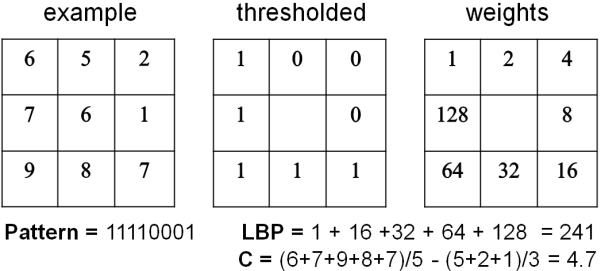
\includegraphics[width=0.8\linewidth]{image004}
\caption{Extraction of LBP features}
\end{figure}

\textbf{Support Vector Machines}\\

Linear support vector machines are originally formulated for binary classification \cite{burges1998tutorial}. Given training data and its corresponding labels , \ensuremath{(x_n,y_n)}, x=1,2..N, ${x_n \in}$ ${\rm I\!R}^D, t_n\in[{-1,+1}]$, SVM's learning consists of the following constrained optimization.\\

\begin{equation*}
\begin{aligned}
 \underset{w, \xi_n}{\text{Min}}
 & & 1/2 w^Tw + C\sum_{n=1}^{N} \xi_n  & & s.t.\\
 w^Tx_nt_n \geq 1 -\xi_n \forall \\
 \xi_n \forall n
\end{aligned}
\end{equation*}

% \begin{itemize}
% \item Bullet point one
% \item Bullet point two
% \end{itemize}

% \begin{enumerate}
% \item Numbered list item one
% \item Numbered list item two
% \end{enumerate}

$\xi_n$ are slack variables which penalizes data points
which violate the margin requirements. Note that we
can include the bias by augment all data vectors $x_n$
with a scalar value of 1. The corresponding unconstrained
optimization problem is the following:



\begin{equation*}
\begin{aligned}
 \underset{w}{\text{Min}}
 & & 1/2 w^Tw + C\sum_{n=1}^{N} max(1-w^Tx_nt_n,0)\\
\end{aligned}
\end{equation*}

The objective of the above equation is known as the primal form
problem of L1-SVM, with the standard hinge loss.
Since L1-SVM is not differentiable, a popular variation
is known as the L2-SVM which minimizes the squared
hinge loss

For Kernal SVMs, optimization must be performed in
the dual. However, scalability is a problem with Kernal
SVMs, and in this paper we will be only using
linear SVMs with standard deep learning models.

\begin{figure}[h]
\centering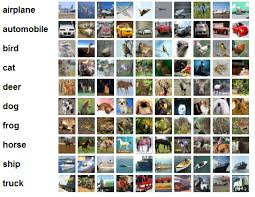
\includegraphics[width=0.8\linewidth]{cifar}
\caption{Multi-Class CIFAR-10 Dataset}
\end{figure}
\textit{Multi-Class SVM's}

The simplest way to extend SVMs for multiclass problems
is using the so-called one-vs-rest approach (Vapnik,
1995). For K class problems, K linear SVMs
will be trained independently, where the data from
the other classes form the negative cases. Hsu and Lin
(2002) discusses other alternative multiclass SVM approaches,
but we leave those to future work.
Denoting the output of the k-th SVM as \\

\begin{center}$a_k(x)=w^Tx$ \\
\end{center}

The predicted class is\\

\begin{equation*}
\begin{aligned}
 \underset{k}{\text{arg max}}
 & & a_k(x)\\
\end{aligned}
\end{equation*}


Note that prediction using SVMs is exactly the same
as using a softmax. The only difference between
softmax and multiclass SVMs is in their objectives
parametrized by all of the weight matrices W. Softmax
layer minimizes cross-entropy or maximizes the
log-likelihood, while SVMs simply try to find the maximum
margin between data points of different classes.\\

The LBP code read in the images and produced feature vectors for each image. Various settings of the LBP code were allowed to answer the following questions:-\\

\begin{enumerate}
\item Is a higher dimensional feature vector more efficient than a lower dimensional one?
\item Would a normalised histogram perform better than an unnormalized one.
\end{enumerate}

We used the LIBSVM MATLAB package for classification. This work addresses the following questions:\\

\begin{enumerate}
\item Which kernel would perform better for higher dimensional features and which kernel for lower dimensional?
\item How much cross-validation is allowed before over-fitting occurs?
\item Figuring out the appropriate cost value for our ideal model?
\end{enumerate}

% \begin{table}[h]
% \centering
% \begin{tabular}{l l l}
% \hline
% \textbf{Treatments} & \textbf{Response 1} & \textbf{Response 2}\\
% \hlinedd
% Treatment 1 & 0.0003262 & 0.562 \\
% Treatment 2 & 0.0015681 & 0.910 \\
% Treatment 3 & 0.0009271 & 0.296 \\
% \hline
% \end{tabular}
% \caption{Table caption}
% \end{table}



% \begin{figure}[h]
% % \centering\includegraphics[width=0.4\linewidth]{placeholder}
% \caption{Figure caption}
% \end{figure}



\section{Experiments}
\label{S:2}


The CIFAR-10 dataset consists of 60,000 images out of which 50,000 are training images and the rest are test data.The number of classes is 10. The images are 32 by 32 and packed in 5 training batches and 1 test batch each of 10,000 images with 1,000 images of each class. This batch format makes it easier in the pre-processing stage. However, much pre=processing of this dataset was still needed; the images were packed in 1-D vectors for compression and they needed to be blown up into proper images to be read by the LBP code.\\

The LBP code is maintained to be rotationally invariant. However, to answer the questions put forth in section 1, we changed the arguments for various settings. The LBP code takes in jpg, png, bmp file formats and the dataset was packed in 1-D uint8 vectors. So we wrote a script to facilitate easy parsing of the dataset for the LBP code.\\

Additionally, LIBSVM only accepts sparse training data of type double. Thus further preprocessing was achieved and the output of the LBP code was packaged in a format easily read by the LIBSVM code. We experimented with numerous settings of the code which are explained below:-\\

\begin{itemize}
\item -t kernel type : set type of kernel function (default 2)\\
	0 -- linear: $U^T*V$ \\
	1 -- polynomial: (*$\gamma*U^T*V$)\\
	2 -- radial basis function: exp$(-\gamma*|u-v|^2)$\\
	3 -- sigmoid: tanh($gamma*u'*v + coef0$)\\
	4 -- precomputed kernel (kernel values in training\_set\_file)\\
\item -c cost : set the parameter C of C-SVC, $\epsilon$\_SVR (default 1)
\item -v n: n-fold cross validation mode
\item -g gamma : set gamma in kernel function (default 1/num\_features)
\end{itemize}

The svmtrain function returns a model which can be used for future
prediction. It is a structure and is organized as Parameters, nr\_class,
totalSV, rho, Label, ProbA, ProbB, nSV, sv\_coef, SVs\\

The function svmpredict has three outputs. The first one,
predictd\_label, is a vector of predicted labels. The second output,
accuracy, is a vector including accuracy (for classification), mean
squared error, and squared correlation coefficient (for regression).
The third is a matrix containing decision values or probability
estimates (if -b 1 is specified). If k is the number of classes
in training data, for decision values, each row includes results of 
predicting k(k-1)/2 binary-class SVMs. For classification, k = 1 is a
special case. Decision value +1 is returned for each testing instance,
instead of an empty vector. For probabilities, each row contains k values
indicating the probability that the testing instance is in each class.
Note that the order of classes here is the same as Label field
in the model structure.\\


\begin{figure}[h]
\centering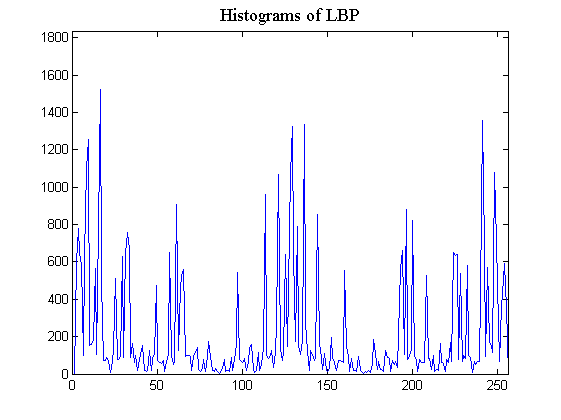
\includegraphics[width=0.85\linewidth]{demo_mlhmslbp_spyr_02}
\caption{Format of output Histogram}
\end{figure}
\textbf{Unnormalised histograms}\\

Various LBP settings were employed. In order to answer the question on normalisation, we trained two models for an unnormalised LBP histogram and 3 models for a normalised histogram. In the unnormalised case, we used an RBF kernel for the first model at a cost of 1 and a gamma of 0.07. The radius was set to 1 and the number of sampling points was 8. For the second model, we switched to a linear kernel with all the LBP parameters remaining same except for the cost which we set to 50. Additionally, we used a 5-fold cross-validation model which took a lot of time.\\

\textbf{Normalised histograms}\\

Testing was switched using normalised histograms. Parameter palettes of 8-point, 16-point and 20-point LBP's were used to check for efficiency of higher dimensional feature vectors. After usage of the RBF kernel in the unnormalised experiment, We tried a sigmoidal (tanh) kernel here but performance was found to be similar. Different cost values were assumed and a range was calculated and experimented with.\\

\begin{figure}[h]
\centering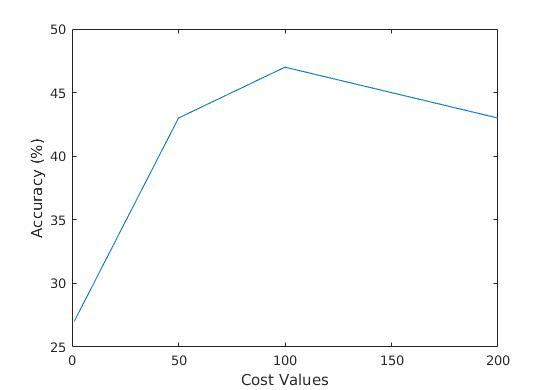
\includegraphics[width=0.85\linewidth]{cost}
\caption{Accuracy vs Cost values}
\end{figure}


\section{Results}
\label{S:2}

\begin{figure}[h]
\centering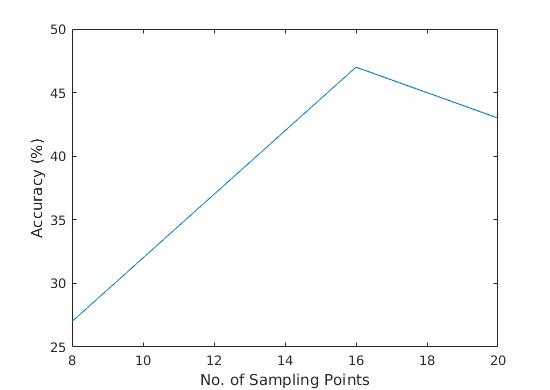
\includegraphics[width=0.85\linewidth]{samplepoints}
\caption{Accuracy vs No. of Sampling Points}
\end{figure}
It is found that a normalised feature vector performs better in general and gives a much wider testbed for further improvements. It gives similar accuracies of 43\% for tanh and sigmoidal kernel functions as well as for the linear kernel with a sampling point of 8. But we have a clear winner with a 16-point sampling range and a linear kernel with a cost of 100 genrating an accuracy of 47\% and a mean squared error of 9.8\% as opposed to the increased 16.55\% that comes with using an RBF kernel. A cost of $>100$ and a sampling point parameter of $>16$ performances sub-optimally at 43/46\% accuracy.\\

\begin{table}[h]
\centering
\begin{tabular}{l l l}
\hline
\textbf{Kernel} & \textbf{Cost\_opt/Points\_opt} & \textbf{Accuracy/MSE/Sq Correlation Coefficient}\\
\hline
RBF (gamma 0.07) & 1/8 & 27\%/16.55/0.03 \\
Sigmoidal & 50/8 & 43\%/-/-(Cross-Validation) \\
Linear & 100/16 & 47\%/9.85/0.15 \\
\hline
\end{tabular}
\caption{Performance of various kernels used}
\end{table}
Additionallly, table one shows that at the specified settings, the linear kernel outperforms the RBF and the sigmoidal kernels. Further testing is required to determine if a larger radius could have a positive effect on the RBF kernel with an improved function for $\gamma$\\ 

Comparison with deep learning techniques shows that CNN's outperform SVM's using LBP features by \~ 30\%. This is evident by the fact that even the most sub-optimally trained model at its worse performs at an accuracy of 53\%. With the most optimally trained CNN performing at 73\%, it is clear that CNN's are the way to go and will dominate the field of computer vision for the forseeable future.

%% The Appendices part is started with the command \appendix;
%% appendix sections are then done as normal sections
%% \appendix

\section{References}
% \label{}

%% References
%%
%% Following citation commands can be used in the body text:
%% Usage of \cite is as follows:
%%   \cite{key}          ==>>  [#]
%%   \cite[chap. 2]{key} ==>>  [#, chap. 2]
%%   \citet{key}         ==>>  Author [#]
%% References with bibTeX database:

\bibliographystyle{plain}
\bibliography{refs}

%% Authors are advised to submit their bibtex database files. They are
%% requested to list a bibtex style file in the manuscript if they do
%% not want to use model1-num-names.bst.
%% References without bibTeX database:

% \begin{thebibliography}{00}

%% \bibitem must have the following form:
%%   \bibitem{key}...
%%

% \bibitem{}

% \end{thebibliography}


\end{document}

%%
%% End of file `elsarticle-template-1-num.tex'.
              